\documentclass[tikz,border=2pt]{standalone}
\usepackage{tikz}
\usetikzlibrary{arrows.meta,calc}

\definecolor{roadgray}{RGB}{211,214,216}
\definecolor{curbdark}{RGB}{86,91,94}
\definecolor{curblight}{RGB}{139,145,148}
\definecolor{egocolor}{RGB}{65,145,162}
\definecolor{targetcolor}{RGB}{232,112,58}
\definecolor{nominalcolor}{RGB}{0,139,151}

% The vehicle drawing is the one used by the ego--obstacle dynamics
% figure, scaled by 0.44 so that its 2.10-unit body length matches the
% 0.924-unit footprint of this scene. The fourth argument steers the
% front wheels. The vehicle longitudinal axis is the local positive x
% direction.
\newcommand{\drawvehicle}[4]{%
    \begin{scope}[shift={(#1)},rotate=#2,scale=0.44]
        % Wheels sit under the body, so they are drawn first.
        \path[fill=black!76]
            (-0.73,-0.60) rectangle (-0.30,-0.43)
            (-0.73,0.43) rectangle (-0.30,0.60);
        \begin{scope}[shift={(0.515,-0.515)},rotate=#4]
            \path[fill=black!76]
                (-0.215,-0.085) rectangle (0.215,0.085);
        \end{scope}
        \begin{scope}[shift={(0.515,0.515)},rotate=#4]
            \path[fill=black!76]
                (-0.215,-0.085) rectangle (0.215,0.085);
        \end{scope}
        \path[
            fill=#3!82,
            draw=black!72,
            line width=0.45pt,
            rounded corners=1.2pt
        ] (-1.05,-0.48) rectangle (1.05,0.48);
        \path[
            fill=white!72!#3,
            draw=black!48,
            line width=0.25pt
        ] (-0.34,-0.37) -- (0.20,-0.37) -- (0.42,-0.27)
          -- (0.42,0.27) -- (0.20,0.37) -- (-0.34,0.37) -- cycle;
        \path[
            fill=black!10,
            draw=black!45,
            line width=0.25pt
        ] (-0.79,-0.34) rectangle (-0.48,0.34);
        \path[fill=white!90!#3,draw=black!45,line width=0.25pt]
            (0.79,-0.27) -- (1.00,0) -- (0.79,0.27) -- cycle;
    \end{scope}%
}


\begin{document}
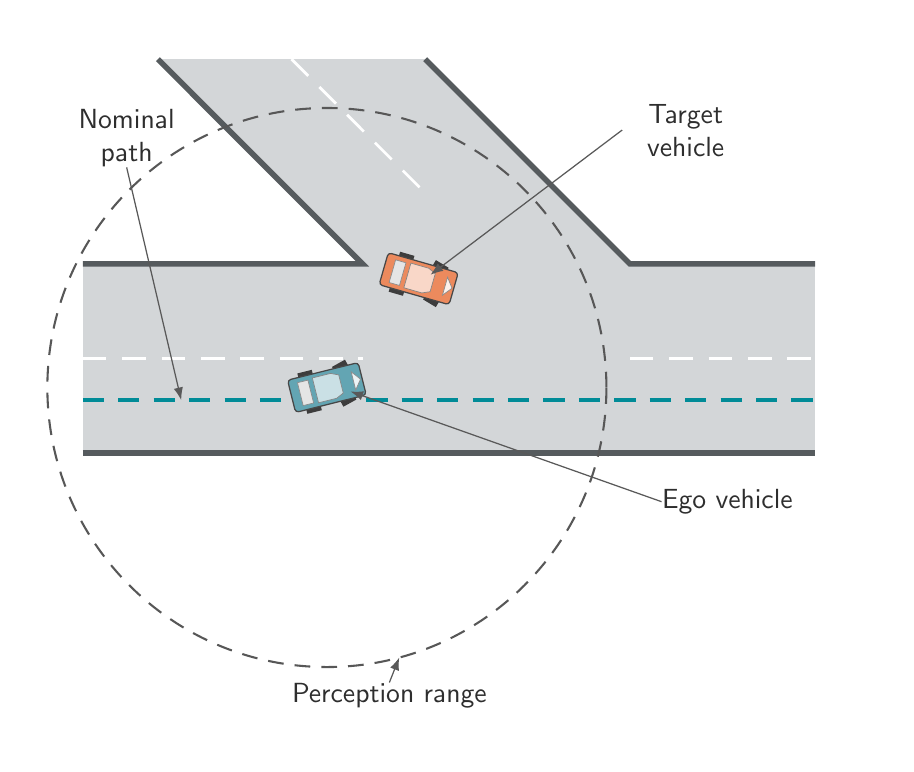
\begin{tikzpicture}[
    callout/.style={font=\sffamily\normalsize,align=center,text=black!82,inner sep=0pt},
    leader/.style={-{Latex[length=1.6mm,width=1.2mm]},draw=black!65,line width=0.45pt}
]
% Design critique: keep. Math/diagram logic review: schematic.
% Exact invariants: Fig. 3 body/wheel angles, equal road widths,
% ego-centered sensing, and an ego footprint within its travel lane.
% Relative centers start from Fig. 3 at scale 0.44; the target is shifted
% slightly downward so its body straddles the side-road mouth.
% The branch is placed around the target in its inbound right-hand lane.
\path[use as bounding box] (-5.45,-4.90) rectangle (5.45,4.20);
\def\egoHeading{14}
\def\targetHeading{-16}
\def\egoSteer{15}
\def\targetSteer{-15}
\def\laneCenterY{-0.53}
\def\roadHalfWidth{1.20}
\def\branchHeading{-45}
\def\branchMouthX{0.50}
\def\branchTopY{3.80}
\def\sensingradius{3.55}
% The ego is displaced toward the lane centerline while keeping its Fig. 3
% heading. Its center does not coincide with the nominal reference path.
\def\egoLateralOffset{0.16}
\coordinate (egoVehicle) at (-1.65,{\laneCenterY+\egoLateralOffset});

% The branch and main road have equal perpendicular width, 2*roadHalfWidth.
\pgfmathsetmacro{\branchHalfMouth}{\roadHalfWidth/abs(sin(\branchHeading))}
\pgfmathsetmacro{\branchLeftMouth}{\branchMouthX-\branchHalfMouth}
\pgfmathsetmacro{\branchRightMouth}{\branchMouthX+\branchHalfMouth}
\pgfmathsetmacro{\branchTopX}{\branchMouthX+(\branchTopY-\roadHalfWidth)/tan(\branchHeading)}
\pgfmathsetmacro{\branchLeftTop}{\branchTopX-\branchHalfMouth}
\pgfmathsetmacro{\branchRightTop}{\branchTopX+\branchHalfMouth}

% Fig. 3 centers: ego (3.75,1.35), target (6.40,5.40).
% Translate the scaled displacement to the off-reference ego center, then
% lower the target by 0.40 drawing units while keeping its rear part in the branch.
\pgfmathsetmacro{\relativeX}{0.44*(6.40-3.75)}
\def\targetDownwardShift{0.40}
\pgfmathsetmacro{\relativeY}{0.44*(5.40-1.35)-\targetDownwardShift}
\coordinate (targetVehicle) at ($(egoVehicle)+(\relativeX,\relativeY)$);

\path[fill=roadgray] (-4.75,-\roadHalfWidth) rectangle (4.55,\roadHalfWidth);
\path[fill=roadgray] (\branchLeftMouth,\roadHalfWidth) -- (\branchRightMouth,\roadHalfWidth)
    -- (\branchRightTop,\branchTopY) -- (\branchLeftTop,\branchTopY) -- cycle;
\draw[curbdark,line width=2.0pt] (-4.75,-\roadHalfWidth) -- (4.55,-\roadHalfWidth);
\draw[curbdark,line width=2.0pt] (-4.75,\roadHalfWidth) -- (\branchLeftMouth,\roadHalfWidth)
    -- (\branchLeftTop,\branchTopY);
\draw[curbdark,line width=2.0pt] (\branchRightTop,\branchTopY)
    -- (\branchRightMouth,\roadHalfWidth) -- (4.55,\roadHalfWidth);
% Center markings stop before the open intersection.
\draw[white,line width=1.0pt,dash pattern=on 3mm off 2mm]
    (-4.75,0) -- (\branchLeftMouth,0);
\draw[white,line width=1.0pt,dash pattern=on 3mm off 2mm]
    (\branchRightMouth,0) -- (4.55,0);
\draw[white,line width=1.0pt,dash pattern=on 3mm off 2mm]
    (\branchTopX,\branchTopY) -- ($(\branchMouthX,\roadHalfWidth)+(135:1.20)$);
% This is the nominal reference, not the maneuvering ego trajectory.
\draw[nominalcolor,line width=1.25pt,dash pattern=on 2.7mm off 1.8mm]
    (-4.75,\laneCenterY) -- (4.55,\laneCenterY);
\draw[draw=black!66,line width=0.75pt,dash pattern=on 2mm off 1.4mm]
    (egoVehicle) circle[radius=\sensingradius];
\drawvehicle{egoVehicle}{\egoHeading}{egocolor}{\egoSteer}
\drawvehicle{targetVehicle}{\targetHeading}{targetcolor}{\targetSteer}

\node[callout,anchor=west,text width=16mm] (targetLabel) at (2.10,2.90) {Target\\vehicle};
\draw[leader] (targetLabel.west) -- ($(targetVehicle)+(0.15,0.05)$);
\node[callout,anchor=west] (egoLabel) at (2.60,-1.82) {Ego vehicle};
\draw[leader] (egoLabel.west) -- ($(egoVehicle)+(0.30,-0.05)$);
\node[callout,anchor=west,text width=16mm] (pathLabel) at (-5.00,2.80) {Nominal\\path};
\draw[leader] (pathLabel.south) -- (-3.50,\laneCenterY);
\node[callout,anchor=west] (rangeLabel) at (-2.10,-4.28) {Perception range};
\draw[leader] (rangeLabel.north) -- ($(egoVehicle)+(285:\sensingradius)$);
\end{tikzpicture}
\end{document}
